\documentclass[journal]{IEEEtran}
\usepackage{amsmath,amsfonts}
\usepackage{amsthm}
\usepackage{booktabs}
\usepackage{array}
\usepackage[caption=false,font=normalsize,labelfont=sf,textfont=sf]{subfig}
\usepackage{textcomp}
\usepackage{stfloats}
\usepackage{url}
\usepackage{verbatim}
\usepackage{graphicx}
\usepackage{amssymb,amsmath,bm} % 移除了空选项[]
\usepackage{siunitx}
\usepackage{arydshln}
\usepackage{enumitem}
\usepackage{gensymb}
\DeclareMathOperator{\flatten}{flatten}
\newtheorem{proposition}{Proposition}


\usepackage{xcolor}
\usepackage{wasysym}
\usepackage[normalem]{ulem}
\usepackage{multirow}
\usepackage{siunitx} 
% \usepackage{graphicx}% <- 重复，请删除此行
% \usepackage{graphics}% <- 重复，请删除此行
% \usepackage{array}% <- 重复，请删除此行
\usepackage{booktabs}
\usepackage{algorithm}
\usepackage{algpseudocode}
\usepackage{cite}

% 正确的加载顺序：先hyperref，后cleveref
%\usepackage{hyperref}
\usepackage[colorlinks, linkcolor=blue, citecolor=blue]{hyperref}
\usepackage{cleveref} % 智能引用

\hyphenation{op-tical net-works semi-conduc-tor IEEE-Xplore}
% updated with editorial comments 8/9/2021

\begin{document}


        % <-this % stops a space
%\thanks{This paper was produced by the IEEE Publication Technology Group. They are in Piscataway, NJ.}% <-this % stops a space
%\thanks{Manuscript received April 19, 2021; revised August 16, 2021.}}
%\thanks{This work was supported in part by the National Natural Science Foundation of China under No. 62271250 and No. U23B2005. ({\it Corresponding authors: Lin Ma})}
% The paper headers


% \IEEEpubid{0000--0000/00\$00.00~\copyright~2021 IEEE}% 
% Remember, if you use this you must call \IEEEpubidadjcol in the second
% column for its text to clear the IEEEpubid mark.



% otgaussvlad for transport-aware global retrieval.
\title{Hierarchical Visual Localization Using otgaussvlad% Time-varying Channel
	
	\thanks{Copyright (c) 20xx IEEE. Personal use of this material is permitted. However, permission to use this material for any other purposes must be obtained from the IEEE by sending a request to pubs-permissions@ieee.org.}
	\thanks{This paper is supported by National Natural Science Foundation of China (62571164). }}

\author{Xiangyun He, Lin Ma, \IEEEmembership{Senior Member, IEEE}, Run Zhang, Yue Yu, Danyang Qin, Mu Zhou, \IEEEmembership{Senior Member, IEEE}
	\thanks{X. He, L. Ma, R. Zhang, Y. Yu are with the School of Electronics and Information Engineering, Harbin Institute of Technology, Harbin, China (e-mail: 24B305050@stu.hit.edu.cn; malin@hit.edu.cn; 25S105173@stu.hit.edu.cn; 24S105182@stu.hit.edu.cn). D. Qin is with the School of Electronics Engineering, Heilongjiang University, Harbin, China (e-mail: qindanyang@hlju.edu.cn). M. Zhou is with the School of Electronic Science and Engineering, Chongqing University of Posts and Telecommunications, Chongqing, China (e-mail: zhoumu@cqupt.edu.cn).(Corresponding author: Lin Ma.)}
	
	
}

% <-this % stops a space
%\thanks{This paper was produced by the IEEE Publication Technology Group. They are in Piscataway, NJ.}% <-this % stops a space
%\thanks{Manuscript received April 19, 2021; revised August 16, 2021.}}

% The paper headers
%\markboth{Journal of \LaTeX\ Class Files,~Vol.~14, No.~8, August~2021}%
%{Shell \MakeLowercase{\textit{et al.}}: A Sample Article Using IEEEtran.cls for IEEE Journals}
\markboth{IEEE Transactions on Image Processing, Vol. XX, No. XX, Month 2024}
{X. He et al.: Hierarchical Visual Localization Using otgaussvlad}
% \IEEEpubid{0000--0000/00\$00.00~\copyright~2021 IEEE}% 
% Remember, if you use this you must call \IEEEpubidadjcol in the second
% column for its text to clear the IEEEpubid mark.






\maketitle


\begin{abstract}
Visual localization in large-scale scenes hinges on the quality of global retrieval. This paper presents otgaussvlad, an optimal-transport-based Gaussian residual aggregator for place recognition. The proposed layer projects backbone tokens into a latent descriptor space, scores them with diagonal-Gaussian energy or normalized cosine similarity, and solves a Sinkhorn transport problem with a learnable dustbin and token-mass prediction. Transport mass is retained at the cluster level and used to build mean and standard-deviation residuals with respect to learnable Gaussian prototypes. The concatenated 2KD-dimensional descriptor is directly $\ell_2$-normalized without an additional projection head. Experiments on Pittsburgh 30k and Aachen Day-Night demonstrate faster convergence and improved retrieval and localization performance over NetVLAD within a standard hierarchical localization pipeline.
\end{abstract}


\begin{IEEEkeywords}
Visual Localization, optimal transport, Gaussian mixture models, Sinkhorn iterations, place recognition.
\end{IEEEkeywords}

\section{Introduction}
%视觉定位，在三维空间中通常对相机进行6DoF定位，这六个自由度分别是三维位移的三个自由度和三维旋转的三个自由度，分别对应定位结果中的三维位置和三轴欧拉角。为在一致的参考系下给出定位结果，6DoF定位需要依赖场景的三维模型，这些模型可由SLAM或SfM得到，SLAM更关注建图的实时性，在建图时会丢弃信息，只选择关键帧用于建图。SfM更关注模型的精度，建图的速度往往会很慢。虽然两类模型都可以使用，但通常来说已知环境对建图实时性需求较小，因此更倾向于使用更为精准的SfM模型。近年来基于场景三维模型的视觉定位方法主要分为了基于直接2D-3D匹配的方法、基于图像检索的方法。%
\IEEEPARstart{V}isual localization typically involves 6 Degrees of Freedom (6DoF) positioning of a camera in three-dimensional space, which encompasses three degrees of freedom for three-dimensional translation and three degrees for three-dimensional rotation, corresponding to the three-dimensional position and three Euler angles in the positioning results. To provide positioning results within a consistent reference frame, 6DoF localization relies on a three-dimensional model of the scene, which can be obtained through Simultaneous Localization and Mapping (SLAM) or Structure from Motion (SfM). SLAM focuses more on the real-time aspect of mapping, discarding information and selecting only key frames for map construction during this process. SfM, on the other hand, places greater emphasis on the accuracy of the model, often at the expense of slower mapping speeds. Although both types of models are usable, in environments where real-time mapping requirements are less critical, there is a preference for the more accurate SfM models. In recent years, visual localization methods based on three-dimensional scene models have primarily been categorized into two approaches: direct 2D-to-3D matching methods and image retrieval-based methods.

%直接2D-3D匹配方法[20][21]是将查询图像提取的特征描述子与场景三维模型中的3D点描述子直接比较得到2D-3D匹配点对。因匹配点对中可能存在部分误匹配，所以会对这些2D-3D匹配点对使用基于随机采样一致性（Random Sample Consensus，RANSAC）的n点透视（Perspective-n-Point，PnP）算法估计相机位姿，以此滤除大部分误匹配点对。这类方法通常需要借助索引技术进行匹配，对于大规模场景且密集描述符的集合中，搜索的时间代价及其昂贵。虽然采取了一系列改进措施[22][23]，但始终在定位精度和效率上存在矛盾。%
Direct 2D-to-3D matching methods involve comparing feature descriptors extracted from query images with those of 3D points in the scene's three-dimensional model to obtain 2D-3D match pairs\cite{ref1,ref2}. Since there may be some incorrect matches among these pairs, a Perspective-n-Point (PnP) algorithm based on Random Sample Consensus (RANSAC) is employed to estimate the camera pose from these 2D-3D matches, thereby filtering out the majority of incorrect matches. These methods typically rely on indexing techniques for matching, which can be computationally expensive, particularly in large-scale scenes with dense descriptor collections. Despite a series of improvements, there remains a trade-off between positioning accuracy and efficiency\cite{ref3,ref4}.

%早期基于图像检索的定位方法是将定位问题视为位置识别问题，以检索得到的最近似数据库图像的位姿作为查询图像的位姿。DenseVLAD和NetVLAD是该类方法的代表。这两种方法都能很好地应对昼夜变化，并且在大规模情况下也能很好工作，但是其定位精度略显不足。现在基于图像检索的方法一般将位置识别与间接2D-3D匹配方法相结合：先对查询图像进行位置识别缩小定位场景范围，再进行2D-2D的匹配以找到2D-3D匹配关系，从而进行精细化的位姿估计。该类方法[24][25]实质用两种方法进行了定位，因此也被称为基于图像检索的分层定位。%
Early image-based localization methods treated the localization problem as a place recognition issue, using the pose of the most similar image retrieved from a database as the pose of the query image. DenseVLAD\cite{densevlad} and NetVLAD\cite{ref7} are representative of such methods. Both are effective in dealing with changes in lighting conditions and perform well in large-scale scenarios, although their positioning accuracy is somewhat lacking. Current image retrieval-based methods typically combine place recognition with indirect 2D-to-3D matching: initially, place recognition is used to narrow down the localization scene, followed by 2D-to-2D matching to establish 2D-to-3D correspondences, leading to refined pose estimation. These methods essentially employ a two-stage process for localization and are thus referred to as hierarchical localization based on image retrieval\cite{ref5,ref6}.


%基于图像检索的分层定位在可扩展性、可靠性和有效性方面展现出显著优势，已成为大规模视觉定位的主流范式\cite{ref6}。然而，该方法性能高度依赖于全局检索阶段的质量：若未能检索到语义一致的局部区域，将导致位姿估计精度显著下降。虽然增加检索图像数量可提高召回率，但计算成本线性增长，阻碍实时应用。在低纹理区域、视角变化或光照变化等挑战性场景下，特征提取的鲁棒性进一步削弱。NetVLAD等全局检索方法\cite{ref7}仅依赖一阶统计聚合，缺乏对局部特征分布差异的显式建模，导致跨季节或跨视角条件下误匹配频发。同时，局部特征提取器面临性能与效率的权衡：SuperPoint\cite{ref8}和DISK\cite{ref9}等模型虽判别性高但计算开销大，而ALIKE\cite{ref10}和XFeat\cite{ref11}等轻量方法因网络结构过度简化，显著性区域感知不足，限制了特征区分性。%
Hierarchical localization based on image retrieval has demonstrated notable advantages in scalability, reliability, and effectiveness, establishing itself as a dominant paradigm for large-scale visual localization\cite{ref6}. However, its performance critically depends on the quality of the global retrieval stage: failure to retrieve semantically coherent local regions leads to significant degradation in pose estimation accuracy. While increasing the number of retrieved images improves recall, it linearly escalates computational costs, hindering real-time applicability. In challenging scenarios such as low-texture areas, viewpoint changes, or illumination variations, the robustness of feature extraction is further compromised. Global retrieval methods like NetVLAD\cite{ref7} rely solely on first-order statistical aggregation, lacking explicit modeling of local feature distribution differences, which frequently causes mismatches under cross-season or cross-view conditions. Meanwhile, local feature extractors face a trade-off between performance and efficiency: models such as SuperPoint\cite{ref8} and DISK\cite{ref9} achieve high discriminability at the cost of substantial computational overhead, while lightweight alternatives like XFeat\cite{ref11} suffer from insufficient salient region perception due to overly simplified network architectures, limiting feature distinctiveness. 

%Therefore, there is an urgent need for a global feature method that takes into account the distribution of local image features. Consequently, there is an urgent need for a sparse local feature extraction method that can meet both timeliness and the ability to identify distinguishable regions.%

To effectively address the aforementioned issues, we have made the following contributions:

(1) We propose otgaussvlad, a global feature aggregation framework that couples diagonal-Gaussian scoring with Sinkhorn transport and a dustbin, thereby producing assignments under explicit mass constraints rather than independent token-wise softmax normalization.

(2) We derive a transport-aware Gaussian residual descriptor that preserves cluster mass, models both mean and scale deviations, and admits a diagonal-Gaussian Wasserstein interpretation of the resulting cluster residuals.

(3) Extensive experiments show that the proposed aggregator improves retrieval accuracy and training stability over NetVLAD while remaining fully compatible with standard hierarchical localization back ends.

\section{Proposed Method}
\begin{figure*}[!ht]
	\begin{center}
		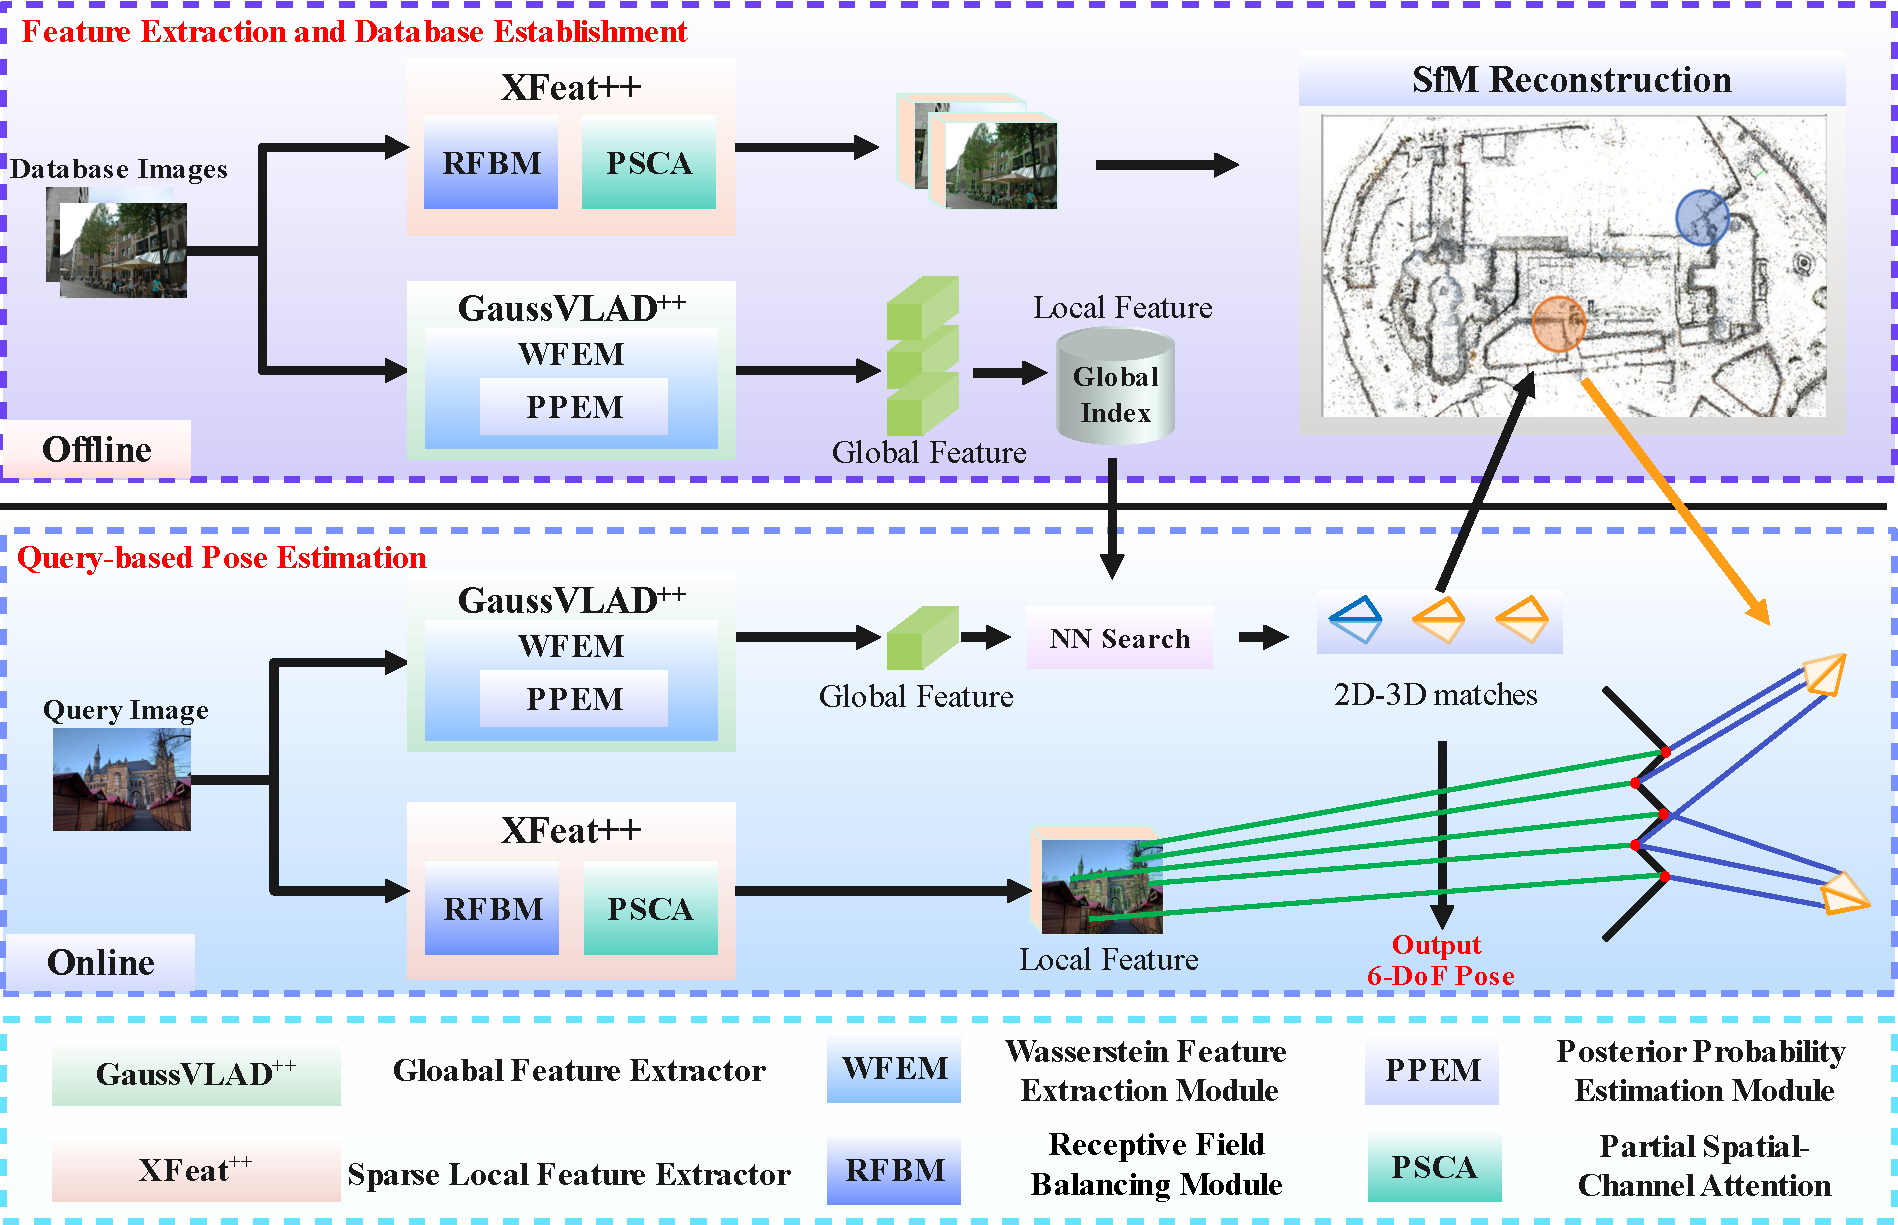
\includegraphics[width=7.1in]{fig1//framework.pdf}
		\caption{Flowchart of the hierarchical visual localization system. The system is divided into two phases: offline and online. In the offline phase, database images are processed by a sparse local feature extractor and otgaussvlad to construct a database containing a global index and a sparse 3D point cloud (SfM Reconstruction). In the online phase, a query image is first processed by otgaussvlad for global retrieval to identify candidate scene regions. Subsequently, sparse local features are matched with the retrieved candidates in a 2D-3D matching step. Finally, the precise 6-DoF camera pose is estimated using a PnP algorithm.}
		\label{framework}
	\end{center}
	\vspace{-0.6cm}
\end{figure*}
\subsection{Framework}
The hierarchical visual localization framework consists of two primary stages: an offline mapping phase and an online localization phase, with the overall workflow illustrated in Fig.~\ref{framework}. The objective of this framework is to efficiently and robustly estimate the 3D position and orientation (6-DoF pose) of a camera based on a single query image.

The core objective of the offline mapping phase is to construct a sparse 3D point cloud model (map) of the target scene and precompute essential features. Specifically, we employ an incremental Structure-from-Motion (SfM) algorithm for 3D reconstruction. This process begins by processing a collection of database images using a sparse local feature extractor and the proposed otgaussvlad global descriptor. The extracted local features are used for feature matching and triangulation steps within SfM to recover the 3D structure and the precise pose for each database image. The global descriptors are also computed and stored. The final mapping results, which encompass the 3D point cloud, the database images' poses, their corresponding local features, and global descriptors, are stored in a database to support efficient online localization.

The online localization phase employs a coarse-to-fine pipeline, comprising three sequential steps. First, in the global retrieval stage, the query image is processed by the otgaussvlad method to extract a global feature descriptor. This descriptor enables rapid similarity computation and K-Nearest Neighbor (KNN) search against precomputed database features, yielding a shortlist of visually similar candidate images. Second, during local feature matching and 2D-3D correspondence establishment, the query and top candidate images are processed by a sparse local feature extractor to obtain local descriptors. Robust 2D-2D feature matching is first established between the query image and candidate database images. These matches are subsequently converted into 2D-3D point correspondences for the query by leveraging the pre-existing associations between 2D keypoints in the candidate images and 3D points in the Structure-from-Motion (SfM) model. Finally, for pose estimation, a RANSAC-based Perspective-n-Point algorithm utilizes the 2D-3D correspondences to estimate the final 6-DoF camera pose. 



\subsection{Transport-Aware Gaussian Residual Aggregator}
Let \(X \in \mathbb{R}^{C \times H \times W}\) denote the backbone feature map. After the two-layer point-wise adapter and LayerNorm, the feature map is reshaped into \(N = HW\) local tokens \(z_n \in \mathbb{R}^D\). In the configuration used in this work, \(C = 768\), \(D = 64\), and \(K = 64\), so the raw descriptor dimension is \(2KD = 8192\). No additional projection head is introduced after aggregation, which keeps the descriptor directly aligned with the residual parameterization.

For each cluster \(k \in \{1,\dots,K\}\), we associate a diagonal Gaussian prototype
\[
p_k(z) = \mathcal{N}(z; \mu_k, \operatorname{diag}(\sigma_k^2)),
\]
where \(\mu_k \in \mathbb{R}^D\) and \(\sigma_k \in \mathbb{R}_+^D\). The mixture prior is parameterized as
\[
\pi_k = \frac{e^{\alpha_k}}{\sum_{j=1}^K e^{\alpha_j}}.
\]
The corresponding Gaussian score, up to a cluster-independent constant, is
\begin{equation}
s_{kn}
= \log \pi_k
-\frac{1}{2}\sum_{d=1}^D \frac{(z_{nd}-\mu_{kd})^2}{\sigma_{kd}^2}
-\sum_{d=1}^D \log \sigma_{kd}.
\label{eq:ot_score}
\end{equation}
For comparison, the attention-based ablation replaces the Gaussian energy with normalized cosine similarity between prototype and token directions, namely \(\bar{\mu}_k = \mu_k / \|\mu_k\|_2\), \(\bar{z}_n = z_n / \|z_n\|_2\), and \(s^{\mathrm{att}}_{kn} = \tau \langle \bar{\mu}_k, \bar{z}_n \rangle\), where \(\tau = \operatorname{softplus}(a) + \epsilon\).

Under the Gaussian mixture model, the posterior responsibility of cluster \(k\) for token \(z_n\) is
\[
r_{kn} = p(k \mid z_n)
= \frac{\pi_k \mathcal{N}(z_n; \mu_k, \operatorname{diag}(\sigma_k^2))}{\sum_{j=1}^K \pi_j \mathcal{N}(z_n; \mu_j, \operatorname{diag}(\sigma_j^2))}.
\]
Equivalently, by Eq.~\eqref{eq:ot_score}, this can be written as
\[
r_{kn} = \frac{\exp(s_{kn})}{\sum_{j=1}^K \exp(s_{jn})}.
\]
This posterior defines the standard token-wise assignment induced by the mixture model. However, it normalizes each token independently and therefore does not impose a global coupling between all tokens and clusters. The transport formulation below can thus be interpreted as a constrained generalization of this posterior assignment.

To encode token relevance, we consider either a uniform mass assignment or a learned one. In the learned case, a token-saliency branch produces logits \(q_n\) and normalized masses
\[
\nu_n = \frac{\exp(\eta q_n)}{\sum_{m=1}^N \exp(\eta q_m)},
\qquad \eta = \operatorname{softplus}(\lambda) + \epsilon.
\]
In the uniform case, \(\nu_n = 1/N\). We denote by \(n = \nu / \|\nu\|_1\) the target marginal.

To attenuate tokens with limited discriminative value, we augment the score matrix with a learnable dustbin row and solve the entropy-regularized transport problem
\[
A^\star = \operatorname*{arg\,max}_{A \in \mathcal{U}(m,n)} \langle \tilde{S}, A \rangle + \mathcal{H}(A),
\]
where \(\mathcal{U}(m,n) = \{A \ge 0 : A\mathbf{1} = m,\ A^\top\mathbf{1} = n\}\), \(\mathcal{H}(A) = -\sum_{k,n} A_{kn}\log A_{kn}\), and
\[
m = \big[(1-\delta)\pi_1,\ldots,(1-\delta)\pi_K,\delta\big]^\top.
\]
Here \(\delta \in (0,1)\) denotes the dustbin mass and \(\tilde{S}\) is the score matrix after appending the dustbin row. This is a finite-dimensional entropy-regularized optimal transport problem. Introducing Lagrange multipliers \(\alpha \in \mathbb{R}^{K+1}\) and \(\beta \in \mathbb{R}^{N}\) for the row and column constraints, the Lagrangian is
\begin{align}
\mathcal{L}(A,\alpha,\beta)
&= \langle \tilde{S},A\rangle \nonumber\\
&\quad - \sum_{k,n}A_{kn}\log A_{kn} \nonumber\\
&\quad + \alpha^\top(m-A\mathbf{1}) + \beta^\top(n-A^\top\mathbf{1}).
\end{align}
Stationarity with respect to \(A_{kn}\) yields
\begin{align}
0 &= \frac{\partial \mathcal{L}}{\partial A_{kn}} \nonumber\\
  &= \tilde{S}_{kn} - 1 - \log A_{kn} - \alpha_k - \beta_n.
\end{align}
Hence,
\begin{align}
A^\star_{kn}
&= \exp(\tilde{S}_{kn} - 1 - \alpha_k - \beta_n) \nonumber\\
&= u_k K_{kn} v_n,
\end{align}
where \(K_{kn} = \exp(\tilde{S}_{kn})\), \(u_k = e^{-1-\alpha_k}\), and \(v_n = e^{-\beta_n}\). Therefore, the optimizer admits the standard matrix-scaling form
\[
A^\star = \operatorname{diag}(u)K\operatorname{diag}(v),
\]
and the corresponding log-space Sinkhorn iterations realize these fixed-point updates in a numerically stable form.

\begin{proposition}[Well-posedness of the transport assignment]
If the source mass \(m\) and target mass \(n\) are strictly positive, then the entropy-regularized transport problem admits at least one maximizer. Because the entropy term is strictly concave on the interior of \(\mathcal{U}(m,n)\), the maximizer is unique.
\end{proposition}
\begin{proof}
The feasible set \(\mathcal{U}(m,n)\) is a transportation polytope. Since \(m\) and \(n\) are probability vectors, the product coupling \(A_0 = mn^\top\) is feasible, because \(A_0\mathbf{1}=m\) and \(A_0^\top\mathbf{1}=n\). The constraints are linear, so \(\mathcal{U}(m,n)\) is closed and bounded in finite-dimensional space and therefore compact. The objective is the sum of a linear score term and the entropy term \(\mathcal{H}(A)\). Since \(-x\log x\) is strictly concave on \(\mathbb{R}_+\), the entropy term is strictly concave on the positive orthant and hence on \(\mathcal{U}(m,n)\). A strictly concave function on a compact convex set admits a unique maximizer. Therefore the entropy-regularized transport assignment is well posed.
\end{proof}

Let \(A\) denote the real-cluster block of \(A^\star\). For each cluster \(k\), define the transported mass
\[
m_k = \sum_{n=1}^N A_{kn},
\qquad
\gamma_{kn} = \frac{A_{kn}}{\max(m_k,\epsilon)}.
\]
If \(m_k > 0\), then \(\sum_n \gamma_{kn} = 1\), and \(\gamma_{k\cdot}\) defines a probability distribution over the tokens assigned to cluster \(k\). The transport-induced empirical moments are then
\begin{align}
\hat{\mu}_k &= \sum_{n=1}^N \gamma_{kn} z_n, \label{eq:mu_hat}\\
\hat{v}_k &= \sum_{n=1}^N \gamma_{kn} (z_n - \hat{\mu}_k) \odot (z_n - \hat{\mu}_k), \label{eq:var_hat}\\
\hat{\sigma}_k &= \sqrt{\hat{v}_k}. \label{eq:sigma_hat}
\end{align}

\begin{proposition}[Transport-induced Gaussian moments]
The quantities \(\hat{\mu}_k\) and \(\hat{v}_k\) are exactly the first and diagonal second central moments of the empirical distribution \(q_k = \sum_n \gamma_{kn}\delta_{z_n}\). Equivalently, \(\hat{\mu}_k\) is the unique minimizer of \(\sum_n \gamma_{kn}\|z_n-\mu\|_2^2\).
\end{proposition}
\begin{proof}
Because \(\sum_n \gamma_{kn}=1\), \(q_k\) is a valid discrete probability measure. Its mean is
\[
\mathbb{E}_{q_k}[z] = \sum_{n=1}^N \gamma_{kn} z_n = \hat{\mu}_k,
\]
which establishes the first identity. To obtain the minimizer characterization, define the weighted quadratic objective
\[
\phi_k(\mu) = \sum_{n=1}^N \gamma_{kn}\|z_n-\mu\|_2^2.
\]
Expanding the square gives
\[
\phi_k(\mu)
= \sum_{n=1}^N \gamma_{kn}\|z_n\|_2^2 - 2\mu^\top\sum_{n=1}^N \gamma_{kn}z_n + \|\mu\|_2^2.
\]
Hence
\[
\nabla_\mu \phi_k(\mu) = 2\Big(\mu - \sum_{n=1}^N \gamma_{kn}z_n\Big),
\qquad
\nabla_\mu^2 \phi_k(\mu) = 2I \succ 0,
\]
so \(\phi_k\) is strictly convex and has a unique minimizer at \(\mu = \hat{\mu}_k\).

For the diagonal second moment, expand the centered square elementwise:
\begin{align}
\hat{v}_k
&= \sum_{n=1}^N \gamma_{kn}(z_n-\hat{\mu}_k)\odot(z_n-\hat{\mu}_k) \nonumber\\
&= \sum_{n=1}^N \gamma_{kn}(z_n\odot z_n) - \hat{\mu}_k\odot\hat{\mu}_k.
\end{align}
This is precisely the elementwise variance of \(q_k\). Therefore \(\hat{v}_k\) and \(\hat{\sigma}_k\) are the diagonal covariance and standard deviation of the transported component.

\end{proof}

The cluster residual is formed as
\[
r_k = [\hat{\mu}_k - \mu_k,\ \hat{\sigma}_k - \sigma_k].
\]
This residual admits a natural interpretation in the diagonal-Gaussian Wasserstein geometry. In particular, once the covariance is expressed through its standard deviation coordinates, the 2-Wasserstein metric becomes Euclidean. The concatenation of cluster-wise residuals therefore yields the final global descriptor.

\begin{proposition}[Wasserstein feature representation]
Using the closed-form 2-Wasserstein distance between Gaussian measures \cite{wgan}, for each Gaussian component the squared 2-Wasserstein distance between the current image component \(X_i \sim \mathcal{N}(\hat{\mu}_i,\hat{\Sigma}_i)\) and the learned prototype component \(Y_i \sim \mathcal{N}(\mu_i,\Sigma_i)\) admits the closed form
\begin{align}
W_2^2(X_i,Y_i)
&= \|\hat{\mu}_i - \mu_i\|_2^2 \nonumber\\
&\quad + \operatorname{Tr}\!\left[\hat{\Sigma}_i + \Sigma_i - 2\left(\hat{\Sigma}_i^{1/2}\Sigma_i\hat{\Sigma}_i^{1/2}\right)^{1/2}\right].
\end{align}
When the covariance matrices are diagonal, write \(\hat{\Sigma}_i = \operatorname{diag}(\hat{\sigma}_i^2)\) and \(\Sigma_i = \operatorname{diag}(\sigma_i^2)\). Since diagonal matrices commute,
\begin{align}
\left(\hat{\Sigma}_i^{1/2}\Sigma_i\hat{\Sigma}_i^{1/2}\right)^{1/2}
&= \operatorname{diag}(\hat{\sigma}_i \odot \sigma_i).
\end{align}
and the trace term reduces to
\begin{align}
\operatorname{Tr}\!\left[\hat{\Sigma}_i + \Sigma_i - 2\left(\hat{\Sigma}_i^{1/2}\Sigma_i\hat{\Sigma}_i^{1/2}\right)^{1/2}\right]
&= \|\hat{\sigma}_i - \sigma_i\|_2^2.
\end{align}
We therefore define the component-wise Wasserstein feature as
\[
g_i = [\hat{\mu}_i - \mu_i,\ \flatten(\hat{\Sigma}_i^{1/2} - \Sigma_i^{1/2})].
\]
For the diagonal case, \(\flatten(\hat{\Sigma}_i^{1/2} - \Sigma_i^{1/2})\) is equivalent to \(\hat{\sigma}_i - \sigma_i\). In this coordinate system, the feature map is an isometric embedding of the diagonal-Gaussian Wasserstein geometry into Euclidean space.

\end{proposition}
\begin{proof}
For the first claim, substitute the diagonal parameterization \(\hat{\Sigma}_i = \operatorname{diag}(\hat{\sigma}_i^2)\) and \(\Sigma_i = \operatorname{diag}(\sigma_i^2)\). Because diagonal matrices commute, the covariance term simplifies to
\begin{align}
\operatorname{Tr}\!\left(\hat{\Sigma}_i + \Sigma_i - 2\left(\hat{\Sigma}_i^{1/2}\Sigma_i\hat{\Sigma}_i^{1/2}\right)^{1/2}\right)
&= \sum_{d=1}^D (\hat{\sigma}_{id}-\sigma_{id})^2 \nonumber\\
&= \|\hat{\sigma}_i-\sigma_i\|_2^2.
\end{align}
Adding the mean term yields
\begin{align}
\|g_i\|_2^2
&= \|\hat{\mu}_i-\mu_i\|_2^2 + \|\hat{\sigma}_i-\sigma_i\|_2^2 \nonumber\\
&= W_2^2(X_i,Y_i),
\end{align}
which proves the first claim.

For the second claim, the prototype component is shared, so the prototype offsets cancel when the two Wasserstein features are subtracted:
\[
g_i - g_i' = [\hat{\mu}_i-\hat{\mu}_i',\ \flatten(\hat{\Sigma}_i^{1/2}-\hat{\Sigma}_i'^{1/2})].
\]
Applying the same diagonal reduction to the pair \((\hat{\mu}_i,\hat{\sigma}_i)\) and \((\hat{\mu}_i',\hat{\sigma}_i')\) yields
\begin{align}
\|g_i-g_i'\|_2^2
&= \|\hat{\mu}_i-\hat{\mu}_i'\|_2^2 + \|\hat{\sigma}_i-\hat{\sigma}_i'\|_2^2 \nonumber\\
&= \|[\hat{\mu}_i-\hat{\mu}_i',\ \hat{\sigma}_i-\hat{\sigma}_i']\|_2^2,
\end{align}
which is exactly the squared 2-Wasserstein distance between the two diagonal Gaussian components. Consequently, concatenating the cluster-wise residuals produces a vector-valued embedding of component-wise Wasserstein discrepancies rather than a scalar distance.
\end{proof}

\noindent\textit{Remark.} In the diagonal parameterization used here, the second coordinate is the standard deviation \(\sigma\), equivalently the square root of the diagonal variance; this is precisely the coordinate system in which the diagonal-Gaussian 2-Wasserstein metric becomes Euclidean.

When \texttt{mass\_preserving} is enabled, the residual is reweighted by
\[
w_k = \left(\frac{K}{1-\delta}m_k\right)^\beta,\qquad \beta = \texttt{mass\_power},
\]
so the final cluster residual becomes \(\tilde{r}_k = w_k r_k\). Since the total real-cluster mass is \(1-\delta\), the factor \(K m_k/(1-\delta)\) measures how much mass cluster \(k\) receives relative to a uniform allocation. The exponent \(\beta\) controls how strongly this occupancy imbalance modulates the descriptor magnitude. This normalization is anchored at the uniform reference mass: if \(m_k = (1-\delta)/K\), then \(w_k = 1\). The final global descriptor is obtained by concatenating \(\tilde{r}_1,\ldots,\tilde{r}_K\) and applying \(\ell_2\) normalization:
\[
g = \frac{\operatorname{vec}([\tilde{r}_1,\ldots,\tilde{r}_K])}{\|\operatorname{vec}([\tilde{r}_1,\ldots,\tilde{r}_K])\|_2}.
\]
Accordingly, the layer may be regarded as a prototype-indexed entropy-regularized transport operator followed by a Wasserstein residual encoder.

\section{Experimental Results and Analysis}
\subsection{Experiment Setup}
This section details the implementation specifics and experimental configurations for the proposed otgaussvlad method. The setup encompasses training datasets, parameter configurations, and hardware/software environments to ensure reproducibility.
\subsubsection{otgaussvlad}
%训练数据集 Pittsburgh 30k \cite{ref7} 包含约 30,000 张来自谷歌街景的带有地理标记的街景图像，其 GPS 坐标精度在 7-15 米以内。捕获时间、视角和光照条件的变化提供了多样化的正样本和困难负样本。
The training dataset, Pittsburgh 30k \cite{ref7}, comprises approximately 30,000 geotagged street-view images from Google Street View, with GPS coordinates accurate within 7--15 meters. Diversity in capture times, viewing angles, and lighting conditions offers a wide range of positive and hard negative samples. Experiments were conducted on a system equipped with an NVIDIA GeForce RTX 4080 GPU and an Intel Core i9-14900K CPU. The software environment included CUDA 12.4, NVIDIA driver version 550.54.14, PyTorch 1.13.0 with CUDA 11.7 support, and torchvision 0.14.0. In the otgaussvlad configuration used in our experiments, the aggregator is instantiated with 768 input channels, 64 clusters, a 64-dimensional cluster space, 768 hidden channels, GMM scoring, three Sinkhorn iterations, a dustbin mass of 0.05, learned token mass prediction, mass-preserving residuals, and mass\_power set to 1.0. This configuration yields an 8192-dimensional global descriptor. The training hyperparameters for both NetVLAD and the proposed otgaussvlad method were identical: an L2 regularization coefficient of 0.001, initial learning rate of 0.0001, learning rate decay rate of 0.5 applied every 5 epochs, momentum of 0.9, and triplet margin threshold of 0.3.


%The objective of global feature extraction is to retrieve database images visually similar to the query, formulated as a supervised learning task using a triplet loss function. Each triplet contains an anchor, a positive sample, and a negative sample. A triplet \((q, \{p_i\}_{i=1}^P, \{n_j\}_{j=1}^N)\) is constructed, where \( q \) represents the query image, the positive sample set \( \{p_i\} \) includes images within 10 meters of the query, and the hard negative set \( \{n_j\} \) comprises images more than 25 meters away. During training, the objective is to minimize the distance between the query image and positive samples while maximizing the distance between the query and negative samples. Since some images in \( \{p_i\} \) may not strictly qualify as positive samples, a weakly supervised triplet loss is applied:
%\begin{equation}
%	\vspace{-0.3cm}
%	\label{eq:3-38}
%	\begin{aligned}
%		L=\sum_j \operatorname{ReLU}\left(\min _i\left\|q-p_i^q\right\|^2 - \left\|q-n_j^q\right\|^2 + m\right) 
%	\end{aligned}
%\end{equation}
%where \( m \) is a margin for distance control. If the distance between the query and positive sample exceeds that between the query and negative sample by \( m \), the triplet loss is set to zero, avoiding penalization for well-separated samples. 



\subsection{otgaussvlad}
%召回率@$K$是全局图像检索的核心指标，用于衡量在前$K$个数据库结果中正确匹配图像的比例。它评估特征编码的效能：高召回率@1反映了顶级精度，而召回率@5及更高阈值表明对光照或视角变化等挑战的鲁棒性。这确保了为后续局部匹配和相机姿态估计可靠地选择候选图像。
\textbf{Metrics.} Recall@$K$ is a core metric for global image retrieval, measuring the proportion of correctly matched images among the top-$K$ database results. It evaluates feature encoding efficacy: high Recall@1 reflects top-tier precision, while Recall@5 and higher thresholds indicate robustness to challenges like illumination or viewpoint variations. This ensures reliable candidate image selection for subsequent local matching and camera pose estimation.
%实验结果清晰地证明了otgaussvlad相较于NetVLAD的显著性能优势。​​ 训练第一轮，otgaussvlad的初始损失值（约0.05）​​，显著低于​​ NetVLAD的损失值（约0.23），​​这表明其在初始表征的优势。其核心优势体现为卓越的收敛速度和最终达到的性能水平：​​ otgaussvlad​​仅需约5个训练周期（epochs），损失值便迅速下降并稳定在接近0.01的极低水平​​，且在后续训练直至第15周期持续保持稳定，损失趋近于0；​​与此形成鲜明对比的是​​，NetVLAD的损失值虽然整体呈下降趋势，但​​收敛速度明显缓慢​​，​​即使经过完整的15周期训练，其最终损失值仍维持在约0.17的水平​​，远未达到令人满意的收敛状态。训练损失曲线的对比​​有力证实​​，otgaussvlad在​​训练效率（收敛速度显著更快）、模型性能（达到并维持更低一个数量级的最终损失）以及训练稳定性方面，所有指标均优于​​NetVLAD。%

\textbf{Results.} Fig.~\ref{loss_vgg} demonstrates otgaussvlad's significant performance advantage over NetVLAD. Initially, otgaussvlad achieves a lower loss (0.05 vs. NetVLAD's 0.23), indicating superior initialization. It converges rapidly, stabilizing near 0.01 after merely 5 epochs and approaching zero by epoch 15. In contrast, NetVLAD exhibits slow convergence, with loss remaining at 0.17 even after 15 epochs. The results confirm otgaussvlad's excellence in training efficiency, model performance, and stability.

\begin{figure}[!ht]
	\begin{center}
		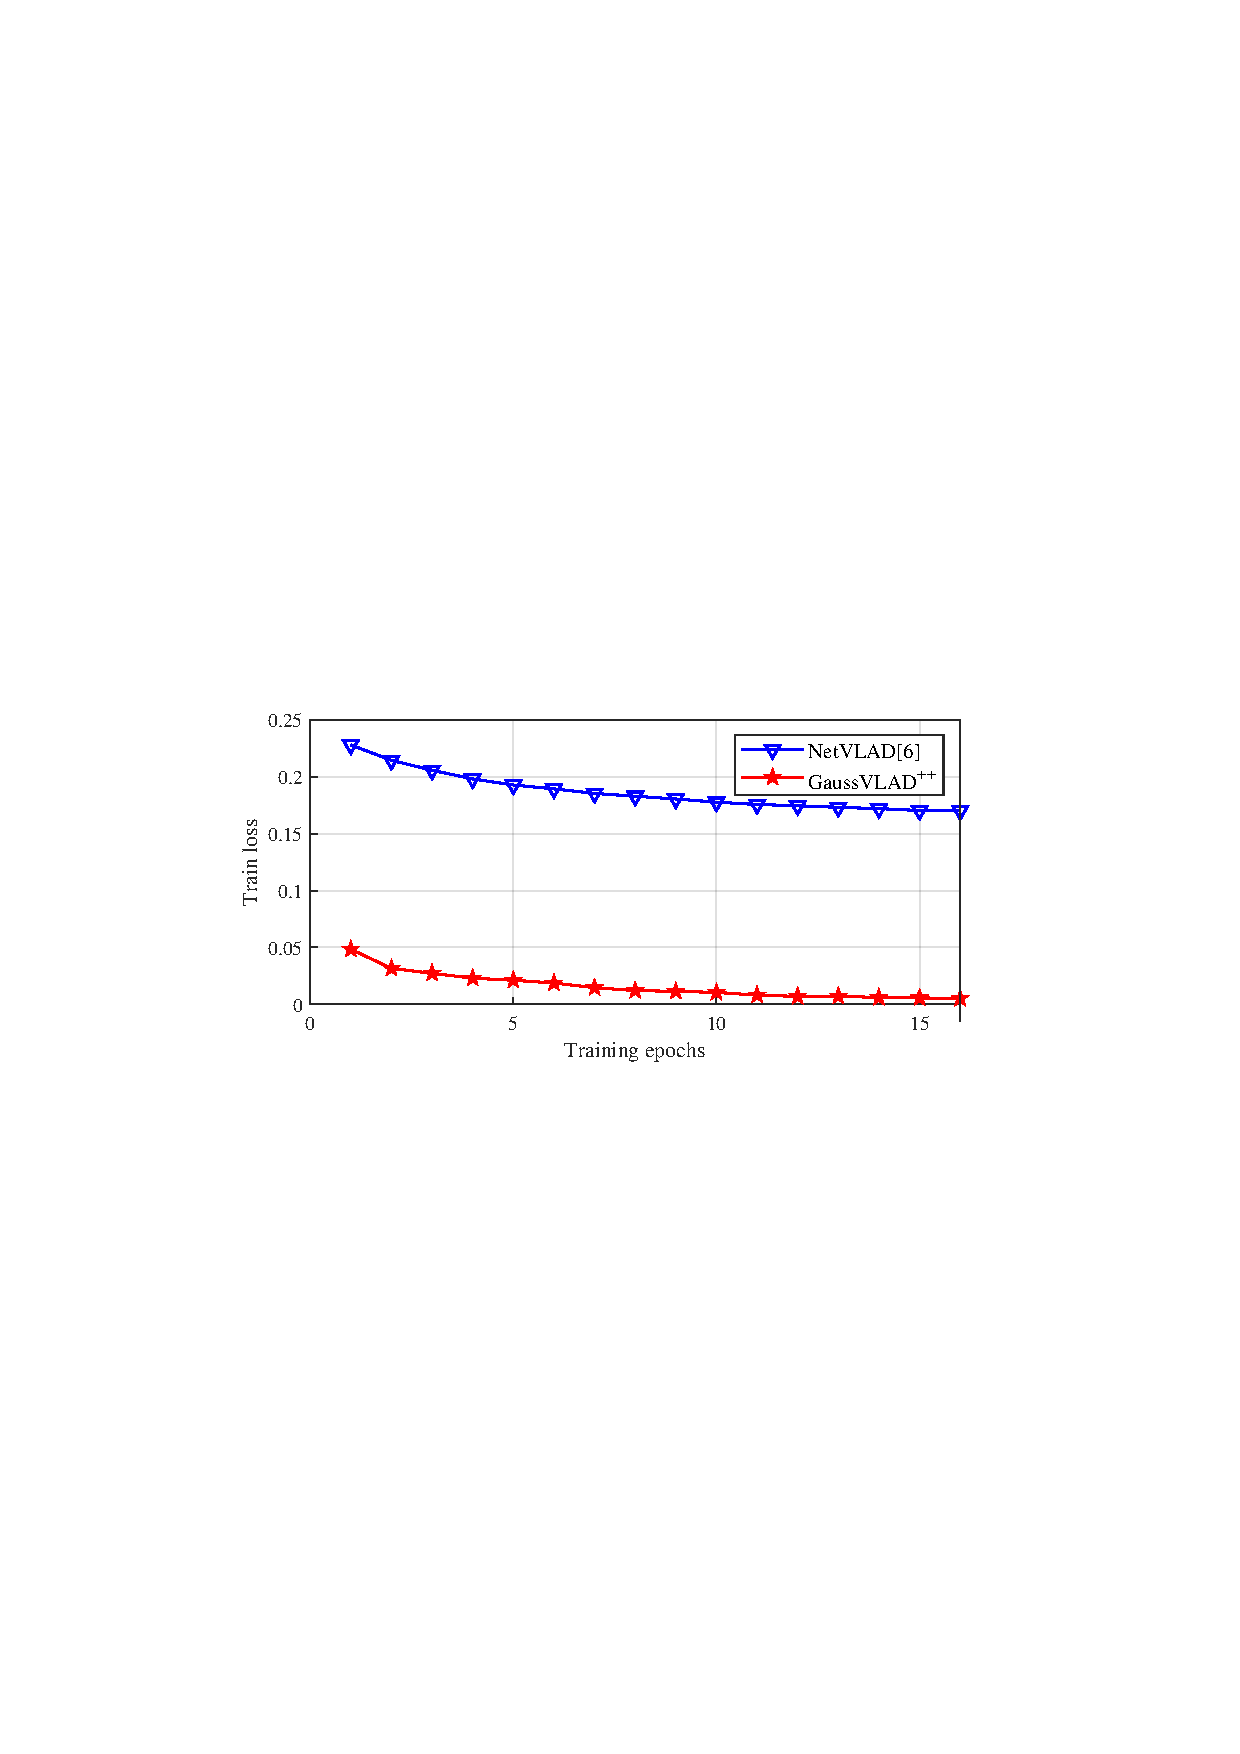
\includegraphics[width=3.4in]{fig1//loss_vgg.pdf}
		\caption{Comparison of training loss over epochs. The graph shows the change in loss during the training process for NetVLAD and otgaussvlad methods. The x-axis represents the number of training epochs, and the y-axis represents the training loss.}
		\label{loss_vgg}
	\end{center}

\end{figure}
%在匹兹堡250k测试数据集上的召回率比较评估总结在表\ref{table:global}中。所提出的基于EfficientNet骨干网络的方法在所有评估指标上均实现了最先进的性能，获得了88.42\%（Recall@1）、95.91\%（Recall@5）、97.39\%（Recall@10）和98.31\%（Recall@20）的召回率。这相对于现有方法有显著提升，在Recall@1上比第二好的方法（MR-NetVLAD）高出1.72个百分点，在更高的召回阈值上高出2.31--2.31个百分点。%
The comparative evaluation of recall rates on the Pittsburgh 250k-test dataset is summarized in Table~\ref{table:global}. The proposed method with an EfficientNet backbone achieves state-of-the-art performance across all evaluation metrics, attaining recall rates of 88.42\% (Recall@1), 95.91\% (Recall@5), 97.39\% (Recall@10), and 98.31\% (Recall@20). This represents a significant improvement over existing approaches, outperforming the second-best method (MR-NetVLAD) by 1.72\% in Recall@1 and by 2.31\% in Recall@5.

%比较结果凸显了骨干网络架构选择的关键作用：基于EfficientNet的变体相比基于VGG的实现展现出显著优势，尤其在Recall@1（提升+4.00\%）和Recall@5（提升+3.17\%）指标上。两种变体均一致超越了NetVLAD基线，验证了所提出特征编码框架在大规模视觉定位任务中的有效性。
The comparison highlights the critical role of backbone architecture selection: the EfficientNet variant exhibits a substantial gain over the VGG-based implementation, particularly in Recall@1 (+4.00\%) and Recall@5 (+3.17\%). Both variants consistently surpass the NetVLAD baseline, validating the efficacy of the proposed feature encoding framework in large-scale visual localization tasks.


\begin{table}[tbp]
	\caption{Comparison of Recall Rates on the Test Set}
	\label{table:global}
	\setlength{\tabcolsep}{3.5pt}
	\centering
	\begin{tabular}{c|cccc}
		\hline
		& \multicolumn{4}{c}{\multirow{1.2}{*}{Pittsburgh 250k-test}}  \\
		\multirow{-2}{*}{Method} & Recall@1 & Recall@5 & Recall@10 &Recall@20\\ \hline
		
		SPE-NetVLAD \cite{ref14}      & 85.60\% & 93.20\% & 94.55\% & 95.90\%  \\
		NetVLAD \cite{ref7} & 81.64\% & 90.98\% & 93.26\% & 95.05\% \\
		MR-NetVLAD \cite{ref17}       &\underline{ 86.70\%} & \underline{93.60\%} & 94.80\% & 96.00\% \\ 
		Ours(VGG)      & 84.42 & 92.74 & \underline{94.87\%} &\underline{96.20\%}  \\
		Ours(EfficientNet)      & \textbf{88.42\%} & \textbf{95.91\%} & \textbf{97.39\%} & \textbf{98.31\%}  \\
		\hline
	\end{tabular}
\end{table}
%为了排除训练框架和骨干网络对模型性能的影响，我们统一使用VGG网络作为Backbone，使用pytorch对NetVLAD和otgaussvlad进行了重新训练。为了验证我们所提的全局检索方法在定位上的有效性，我们在固定稀疏局部特征和特征匹配方法的情况下，使用hierarchical localization toolbox（Hloc）评估我们所提方法otgaussvlad在定位方面所产生的作用。正如表\ref{tab:globalfeatures}所示，结果表明我们所提方法对于白天和夜间的图像都能召回与查询图像相关性很高的数据库图像。这个结果正如我们设计otgaussvlad的本质一样，使用协方差矩阵建模特征之间的相关性，采用Wassertain距离作为特征相似性度量，更好的考虑了局部语义特征的分布，使提取的全局特征在召回候选图像时更加具备优势。%
To eliminate the impact of the training framework and backbone network on model performance, we uniformly used the VGG network as the Backbone and retrained NetVLAD and otgaussvlad using PyTorch. To verify the effectiveness of our proposed global retrieval method in localization, we evaluated the role of our method otgaussvlad in localization using the hierarchical localization toolbox (Hloc) under fixed sparse local features and feature matching methods. As shown in Table \ref{tab:globalfeatures}, the results indicate that our method can recall database images highly relevant to the query images for both daytime and nighttime scenes. This outcome aligns perfectly with the essence of our design for otgaussvlad, which employs the Wasserstein distance as a measure of feature similarity. This approach better considers the distribution of local semantic features, giving the extracted global features a significant advantage when retrieving candidate images.

\begin{table}[htbp]
	\centering
	\caption{Performance Comparison of Global Feature extracting Methods on Aachen Day-night}
	\label{tab:globalfeatures}
	\setlength{\tabcolsep}{2.5pt}
	\begin{tabular}{lccc ccc}
		%\toprule
		\hline
		\multirow{3}{*}{\centering Method} & 
		\multicolumn{3}{c}{\multirow{1.5}{*}{Day}} & 
		\multicolumn{3}{c}{\multirow{1.5}{*}{Night}} \\
		\cmidrule(lr){2-4} \cmidrule(lr){5-7}
		& 0.25m 2° & 0.5m 5° & 5m 10° & 0.25m 2° & 0.5m 5° & 5m 10°\\
		
		%\midrule  
		\hline
		
		NetVLAD \cite{ref7} & \underline{81.6} & \underline{87.4} & \underline{92.0} & \underline{71.4} & \underline{81.6} & \underline{91.8} \\
		otgaussvlad &  \textbf{83.1} &  \textbf{89.9} &  \textbf{93.9} &  \textbf{79.6} &  \textbf{87.8} &  \textbf{94.9} \\
		
		
		%\bottomrule
		\hline
	\end{tabular}
\end{table}


\section{Conclusion}
This paper presents otgaussvlad, a transport-aware global feature aggregator for hierarchical visual localization. By combining diagonal-Gaussian scoring, Sinkhorn transport with a dustbin, learned token mass, and mass-preserving mean/scale residuals, the proposed layer produces a compact descriptor that is more robust to appearance variation than NetVLAD while remaining fully compatible with conventional retrieval-and-matching pipelines. Experiments on Pittsburgh 30k and Aachen Day-Night confirm faster convergence and improved retrieval and localization performance.

\bibliographystyle{IEEEtran}
%\bibliography{new}
%\begin{thebibliography}{1}
%	\bibliographystyle{IEEEtran}

	
\bibliographystyle{IEEEtran}
\bibliography{ref}


	


%\end{thebibliography}





\end{document}


Therefore, the layer can be viewed as a prototype-indexed entropy-regularized transport operator followed by a Wasserstein residual encoder.
